\documentclass{IEEEtran}
\usepackage[utf8]{inputenc}
\usepackage[english]{babel}
\usepackage{listings}
\lstset{
    language=python,
    basicstyle=\small\ttfamily,
    frame=tb,
    showstringspaces=false
}
\usepackage{hyperref}
\usepackage{amsmath}
\usepackage{graphicx}
\usepackage{csquotes}
\renewcommand{\mkbegdispquote}[2]{\itshape}
\usepackage{multirow}
\usepackage{graphics}
\graphicspath{{./images/}}
\usepackage[style=nature]{biblatex} \addbibresource{references.bib}

\title{Assessing quality of music generated by the Music Transformer with an
American Folk dataset \\
\normalsize{\url{github.com/gregwinther/folk_transformer} and
\url{https://gregwinther.github.io/folk_transformer/}}}

\author{
    \IEEEauthorblockN{Sebastian G. Winther-Larsen} \\
    \IEEEauthorblockA{\textit{Center for Computing in Science Education,
        Department of Physics, University of Oslo} \\
    }
    \and
    \IEEEauthorblockN{Tom F.Hansen} \\
    \IEEEauthorblockA{\textit{Institute of Informatics, University of Oslo} \\ }
    \and
    \IEEEauthorblockN{Bjørn Iversen} \\
    \IEEEauthorblockA{\textit{Institute of Informatics, University of Oslo} \\ }
}


\begin{document}

\maketitle

\begin{abstract}
    Since the publication of the music transformer in 2017,
    music generators based on machine learning (ML) with the transformer architecture 
    has been state of the
    art, making it possible to generate realistic music for over a minute. Up to now
    the results have mainly been succesful for classical piano music, but have failed for
    more technically complex music such as jazz. Americana folk music can be seen
    as a stepping stone to more complex music. In this work we generate Americana
    folk music with 2 different approaches; transfer learning from the MAESTRO
    dataset and solely training on a dataset of Americana music.
    Moreover, we propose
    a framework for the evaluation of these results in a quantitative and
    qualitative way, leaning on Evidence-Based Design 
    for Assessment and Evaluation. Results from the quality
    assessment indicate that both models have been moderately succesful, and the
    model based on transfer learning is favoured. In a rating process people have
    rated the songs to in average 2.6, where 1 is not realistic and 5 is
    realistic.
\end{abstract}

\begin{IEEEkeywords}
    music generation, transformer model, evaluation,
    transfer learning, Americana
\end{IEEEkeywords}

\section{Motivation and introduction}

The attention-based transformer model \cite{vaswani2017attention}, is today
recognised as the best performing sequential machine learning model,
surpassing RNN-based models in most cases, mainly because of its
superior memory efficiency and shorter training because it is parallelizable.
While originally applied to natural language processing (NLP),
which today has mature implementations,
the architecture can also be applied for other sequential learning tasks,
such as music generation~\cite{huang2018music}. The music transformer
developed in the Magenta project is trained on the MAESTRO
dataset~\cite{maestrodataset}. By setting a primer – a start music sequence,
the model generates new music with good results along the same lines as the
training set. With other primers than the regular and systematic classical
music in MAESTRO, the quality of the output is varying.

A \textbf{main goal} of this work is to describe a framework for the quality assessment of different
approaches to the generation of music with the transformer model. This is further
motivated by the attempt to generate, and hence evaluate, more varied music than 
up to now has been successfully generated. We compare
two different Transformer implementations and use our proposed evaluation
framework to assess the quality of each approach. At the core of such an evaluation framework
is an evaluation format that combines a form of quantitative and qualitative evaluation technique. 
In ML-modelling dealing with a creative art like music, the subjective 
experience of the result will be an important part in the evaluation, hence the importance of increasing 
the evaluation scheme from the purely technical approach that is normal for most 
ML-models.

To this end, we wish to employ the transformer music model to a subgenre of music
to which such a model has not been extensively applied. Initial findings from
applying the transformer to jazz music has shown some
limitations~\cite{wu2020jazz}, applying LSTM networks to Blues has been
moderately succesful~\cite{eck2002bluesLSTM} and applying the transformer
model to pop piano music seems to work well~\cite{huang2020pop}. This may be due 
to the rules and structure of pop and classical music - classical music often 
has formal rules, the epitome of which is the fugue~\cite{giraud2015computational}; and
pop music follows some very clear norms~\cite{hennion1983production}. While
even Free Jazz has \emph{some} rules, it readily falls into the category of
the type of rhythmic music with the least amount of structure, that it is
``characterized by the absence of set chord patterns or
time patterns''\cite{FreeJazz}.

American roots music, encompassing spirituals, cajun music, cowboy music,
work songs, but also early blues such as Dixieland; from now on referred to
as ``Americana'', presents itself as hitherto unexplored territory. It also
provides a nice stepping stone towards more ``unstructured'' music as it
often allows for improvisation, but otherwise retains a relatively rigid
structure~\cite{libcong}. We have therefore collected a dataset of MIDI files
of Americana music, which we will use in our quality assessment framework.
A \textbf{secondary goal} is therefore to realistically generate Americana music with the 
transformer
architecture. A natural \textbf{third goal} in the process-steps is to investigate the
superiority of music generators based on a significantly higher number of
songs, even though this could be music from other genres, by utilizing
transfer learning from the MAESTRO dataset in the music transformer
\cite{huang2018music}.

In the next chapter (II) we present related work that we have elaborated on, both
dealing with music generation and music evaluation. Chapter III deals with methods  
used for evaluation and modelling. In chapter IV we describe the 2 musical datasets.
Chapter V and VI describes results and discussion, before chapter 7 illustrate 
challenges and sum up conclusions.

\section{Related work}

The transformer model is considered state of the art
in music generation, surpassing RNN-based models in the last few years. Both
are sequential models, but the attention principle at the core of the
transformer facilitates remembering coherence over longer sections of
sequences and highlights especially important sections. From generating music
of 10s of seconds with RNNs, it is now possible to generate a minute of
coherent realistic music~\cite{huang2018music}. Still, there are a lot of
unresolved challenges, like generating long sections over some minutes, in
highly irregular compositions and multi-channel or many-instrumental signals.
To combat these challenges the improvement of the transformer model has a high
focus in the research community. Some of the most recent attempts are the
Transformer-XL~\cite{dai2019transformerxl} and the
Reformer~\cite{kitaev2020reformer}.
The Reformer claims to be trained on a standard computer with a single GPU.
In this analysis, we will utilize and adaption of the Transformer-XL
architecture for music.

\subsection{Music transformers}

In the existing papers considering music
generation Transformer models we want to emphasize some important related
works besides the aforementioned music transformer, built on the classical
piano music dataset MAESTRO. These works are somewhat diversified in
different music genres, describing the span of existing music genres
generated by the transformer, "setting the stage" for the Americana music in
this work. In the pop music transformer \cite{huang2020pop} pop piano music
is generated by the transformer, a setting quite similar to the classical
piano music in the music transformer \cite{huang2018music}.

Increasing the complexity of music generated, \citeauthor{wu2020jazz} describes
the Jazz transformer which is in
the other end of the spectrum related to complexity. Here the
Transformer-XL architecture is utilized to model lead sheets of jazz music.
Moreover, the model endeavours to incorporate structural events present in the
Weimar Jazz Database (WJazzD) for inducing structures in the generated music, 
the results are not impressive according to subjective listening tests and technical 
evaluation based on pitch class histogram entropy.
Listening tests shows a clear gap between the ratings of the generated and
real compositions. The work analyses the missing parts and presents a
prediction system which analytically shed light on why
machine-generated music to date still falls short of the artwork of humans.
This includes analyzing the statistics of the pitch class, grooving, and
chord progression, assessing the structures of the music with the help of
the fitness scape plot, and evaluating the model’s understanding of Jazz
music. The evaluation scheme and the failure to generate such complex music
is relevant in the generation of Americana.

In a system called LakhNES,
multi-instrumental music is generated with a Transformer~\cite{donahue2019lakhnes}.
Their success of music generation with the piano score generation is
partially explained by the large volumes of symbolic data readily available
for that domain. They leverage the recently-introduced NES-MDB dataset of
four-instrument scores from an early video game sound synthesis
chip\footnote{The Nintendo Entertainment System (NES)}. They found this data
to be well-suited to training with the Transformer architecture. The model
was further improved with a pre-training technique to leverage the
information in a large collection of heterogeneous music, namely the Lakh
MIDI dataset. By performing transfer learning on the NES-MDB dataset, both
the qualitative and quantitative performance from the target dataset was
significantly improved. The rare use of transfer learning in music generation
with the transformer is a relevant foundation for use of transfer learning in
this work.

\citeauthor{gan2020foley} use the transformer architecture to generate music,
but with another approach. In a system called Foley Music, they synthesize
music from a silent video about people playing
instruments~\cite{gan2020foley}. A relationship between body keypoints and
classical MIDI recordings is established. Music generation is then formulated
as a motion-to-MIDI translation problem, represented with a graph transformer
framework that predicts MIDI from motion. By testing the generator on
different music performances the results are proven to outperform several
existing systems in music generation, again for classical music, but now not only piano music.

Summarized there are a few examples of successfully generating music with the transformer,
mainly with classical music. However, there is little work on 
generating intentionally the same music generator with different approaches, 
as will be the case in our work. Another new approach is to use transfer
learning from an existing high-performance music model, opposed from the 
"simpler" NES-MDB dataset.

\subsection{Evaluation of AI-generated music}

In the evaluation of music generation models based on machine learning we would like to point out the
works by \citeauthor{yang2020evaluation}~\cite{yang2020evaluation} describing the technical 
evaluation system mgeval, utilized in this work,
\citeauthor{wu2020jazz}~\cite{wu2020jazz} describing a system of qualitative listening 
tests and 5 objecitive measurements of the structure in the music, and lastly the qualitative 
evaluation measures carried out by \citeauthor{sturm2017taking}
\cite{sturm2017taking}, focusing both on qualitative interviews and statistics about the 
generated notes. These works describe qualitative and quantiative evaluations
between \textbf{real music and a generated music}. In this work we elaborate
on these works and combine approaches in a proposal of a common framework for evaluating
\textbf{different} transformer models for music generation.

\section{Methods}

Acting as a base and for exemplification of the benchmark architecture,
Americana music is generated in 2 different model concepts:
\begin{enumerate}
    \item Utilize transfer learning with MAESTRO music transformer as a base,
        and train with the full dataset of Americana music.
    \item Train a new transformer model only with the full
        Americana dataset.
\end{enumerate}

We hypothesise that the transfer learning model will result in the best
performing
model, but an important issue is what makes up the best model and how to
evaluate such a subjective "sequence-result" as music in a fair and
trustworthy manner. The objective is to investigate if the transfer learning 
model is performing significantly better than a model only trained on
a single dataset, such as has been shown in other ML applications, like image
classification~\cite{7404017}, even though the MAESTRO dataset is totally
different from the Americana dataset.

An attempt to sort this out is by evaluating in a quantitative and
qualitative way, as will be the charecteristics in our work. 
The quantitative, hence objective, way can shortly be
described as a technical comparison of the predicted signal and the real
signal. Principles by \citeauthor{yang2020evaluation}~\cite{yang2020evaluation}
and \citeauthor{wu2020jazz}~\cite{wu2020jazz} will be utilized, further described 
in the section below.

The qualitative part constitutes a music expert judgement, based on listening
to the generated music files from the objective evaluation. In a second, and
survey-based part, 12 random persons are asked to rate the different
music files.

\subsection{Qantitative evaluation}

For quantitative evaluation, we will be using the objective evaluation
toolbox \lstinline|mgeval|~\cite{yang2020evaluation}.
The toolbox extracts absolute
metrics from MIDI files, which allows for inspection of properties of the
dataset used for training and the generated dataset. The features extracted
for absolute measures are divided into pitch-based features:
\begin{itemize}
    \item Pitch count (PC)
    \item Pitch class histogram (PCH)
    \item Pitch class transition matrix (PCTM)
    \item Pitch range (PR)
    \item Average pitch interval (PI)
\end{itemize}

and rhythm-based features:

\begin{itemize}
    \item Note count (NC)
    \item Average inter-onset-interval (IOI)
    \item Note length histogram (NLH)
    \item Note length transition matrix (NLTM)
\end{itemize}

These metrics can then be used to
acquire the relative metrics between datasets with the use of exhaustive
cross-validation to acquire the distance between each sample of the same set
(intra-dataset) and another set (inter-dataset).

\subsection{Evidence-Based Design for Assessment and Evaluation}

As a rigorous and well-proven approach do construct a framework for assessing
music composed by artificial intelligence models, we propose adapting the
methodology of Evidence-Centered
Design~\cite{mislevy2003focus,mislevy2017evidence}.
By working with
Evidence-Centered Design (ECD), we engage in a modern approach to assessment
design, and for assessing complex knowledge and practices. ECD is originally
applied to the contruction of psychometric learning assessment tools. Through
to completion, it would take several years to construct such a tool,
something that is well outside the scope of this study. However, we prospose
to begin with the first step within ECD - \textbf{Domain Analysis}. This
involves exploratory interviews of experts in the field in order to contruct
a thematically organized and prioritized list of knowledge and practices to
assess. Specific to our study, we find it necessary to talk to professional
musicians and composers in order to uncover what actually makes a good
composition.
The method described has similarities with studies performed by \citeauthor{sturm2017taking}
\cite{sturm2017taking}.

To supplement the qualitative evaluation a survey was distributed to
random people with unknown backgrounds. The participants were presented to 5
generated songs with length between 40 seconds and one minute,
facilitated in a Google survey form.
The songs were generated by sending a primer of the first three bars
(five seconds) of five different original songs from the Americana dataset to the
trained model. Each song were presented in two versions, one generated by
Transfer-Americana and one by Americana. The participants had to choose the one they
liked best in each pair of songs. In addition they had to rate the best
version related to how realistic it was compared to human generated music.
The range was 1 (worst) to 5 (best).

\subsection{Modelling process}

MIDI-files was first preprocessed to fit into
the format used by the transformer model. This was carried out by utilizing
an implementation of a transformer-XL~\cite{dai2019transformerxl}, adapted for 
music, incorporated in a
package called Musicautobot~\cite{musicautobot}. Scripts for transfer learning
and single learning were built around this package. Both models had the same
model topology, used the same tuning parameters, and were trained on 
four NVIDIA 2080TI GPUs at University of Oslo for approximately ten 
hours each. The models had the following parameters, \lstinline|n_layers|=16
\lstinline|d_model| = 512, \lstinline|d_head| = 64,
\lstinline|n_head| = 8, \lstinline|d_inner| = 2048, \lstinline|mem_len| = 512,
and \lstinline|batchsize| = 8.

\section{Datasets}

A brief summary of each of the datasets we have used in this study can be
found in \autoref{tab:data}.

MAESTRO~\cite{maestrodataset} (MIDI and Audio Edited for Synchronous
TRacks and Organization) is a dataset with over 200 hours of virtuosic piano
perfomances captured with a fine alignment of approximately 3ms between note
labels and audio waveforms.

The data is a product of performances in the International
Piano-e-competition. During each installment of the competiton, virtuoso
pianists perform on Yamaha Disklaviers which, in addition to being
concert-quality acoustic grand pianos, utilize integrated high-precision MIDI
capture and playback.

Since the MAESTRO dataset contains MIDI recordings from competions,
the pieces are from a select set for each year. This means that many of the
pieces are the same, but may includes much variation within each performer's
interpretation of the piece.

The Americana dataset is constructed from musical scores by Benjamin
Robert Tubb \footnote{sourced online}. These
scores are in the public domain and composed between the ealry 1800s and
1922. The genres range from blues, ragtime, naval songs, hyms, minstrel songs
and spirituals.

\begin{table}
    \begin{center}
    \caption{
        Data set description.
        \label{tab:data}
    }
    \begin{tabular}{l c c c} \hline
            & MAESTRO v2 & Americana \\ \hline\hline
        No. of songs & 1282 & 5711 \\ \hline
        Total time [hours] & 201 & 329 \\ \hline
        Mean length [min] & 9.4 & 3.45 \\ \hline
    \end{tabular}
    \end{center}
\end{table}


\section{Results}

\subsection{Quantitative evaluation}

\begin{table}
    \begin{center}
    \caption{
        Results from relative measurements of Intra-set distances.
        \label{tab:q_results}
    }
    \begin{tabular}{l|rr|rr|rr}
        \multirow{3}{*}{} & \multicolumn{2}{c|}{Training}
            & \multicolumn{2}{c|}{Americana} & \multicolumn{2}{c}{Transfer} \\
        \cline{2-7} & \multicolumn{2}{c|}{Intra-set} & \multicolumn{2}{c|}{Intra-set}
            & \multicolumn{2}{c}{Intra-set} \\
        \cline{2-7} & \multicolumn{1}{c|}{mean} & \multicolumn{1}{c|}{STD}
            & \multicolumn{1}{c|}{mean} & \multicolumn{1}{c|}{STD} 
            & \multicolumn{1}{c|}{mean} & \multicolumn{1}{c}{STD} \\ \hline
        PC & 11.777 & 1.700 & 3.577 & 0.636 & 6.466 & 0.706 \\
        NC & 442.377 & 73.911 & 11.377 & 1.542 & 21.955 & 4.678 \\
        PCH & 0.384 & 0.013 & 0.164 & 0.007 & 0.365 & 0.026 \\
        PCTM & 821.396 & 56.336 & 10.475 & 0.292 & 25.991 & 3.303 \\
        PR & 19.088 & 1.638 & 5.266 & 0.611 & 10.400 & 2.038 \\
        PI & 3.836 & 0.510 & 0.848 & 0.128 & 2.032 & 0.479 \\
        IOI & 0.046 & 0.006 & 0.105 & 0.007 & 0.235 & 0.022 \\
        NLH & 0.471 & 0.027 & 0.263 & 0.022 & 0.466 & 0.043 \\
        NLTM & 316.896 & 23.442 & 23.241 & 1.359 & 46.778 & 4.027
    \end{tabular}
    \end{center}
\end{table}

\begin{figure}
    \centering
    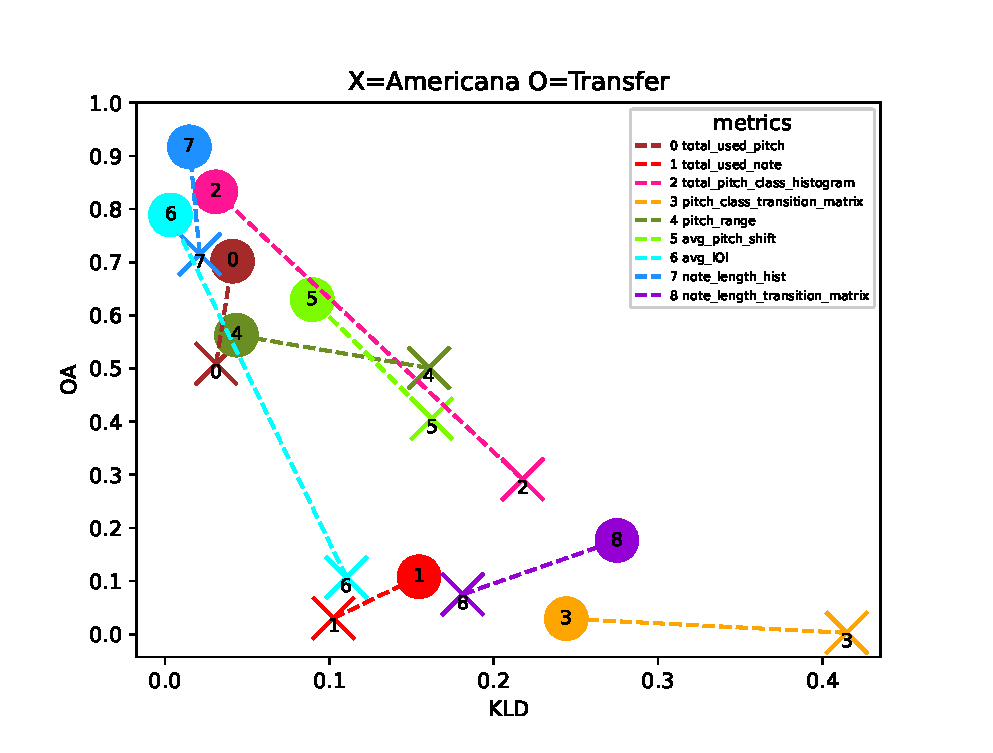
\includegraphics[width=0.485\textwidth]{gen_intra_gen_training_inter}
    \caption{
        Visualisation of the KLD and OA of the Intra-set generated from
        Training set and the American/Transfer sets.
        \label{fig:gen_intra_gen_training_inter}
    }
\end{figure}

\begin{figure*}
    \centering
    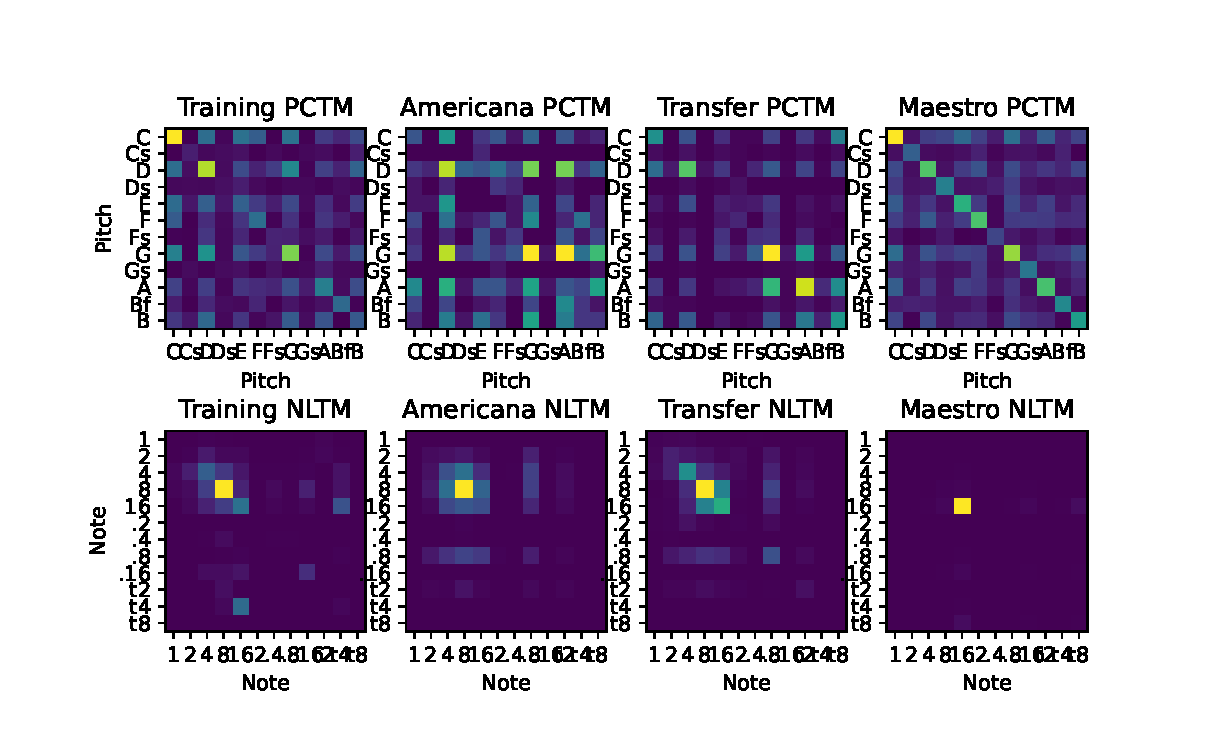
\includegraphics[width=0.9\textwidth]{PCTMNLTM.eps}
    \caption{
        Absolute measurements of average pitch class transition matrix
        (PCTM) and note length transition matrix (NLTM) from the Americana
        training set, Americana generated, transfer generated and MAESTRO
        training set (sect IV.A.)
        \label{fig:absoluteNLTMPCTM}
    }
\end{figure*}

For this evaluation we have picked ten melodies from both the Americana
dataset and the MAESTRO dataset, as well as using ten different primers to
generate ten melodies with the Americana trained and the transfer trained
melody sets. The first  five melodies, denoted 0-4, is generated by the
same primers as in the survey melodies visualized in \autoref{fig:songs}.

The results for the absolute measures of note length transition matrix
in \autoref{fig:absoluteNLTMPCTM} shows us that the Americana/training dataset have
a greater variety in note length than the MAESTRO set (comparing similarity 
between column 1 and 4). We can see that the
melodies generated with the Americana dataset have similar variety and that
the melodies generated with the Transfer set influenced by the MAESTRO set preservers
most variety (comparing column 2 and 3 with the real melodies in column 1). 
The result for pitch class transition matrices on the other
hand shows a decrease in variety in the transfer generated melodies.

The results for the relative measurements shown in \autoref{tab:q_results}
and \autoref{fig:gen_intra_gen_training_inter}. From the comparisons we
can see that both the Americana and Transfer sets have notably smaller mean
values in the Intra-set across the board, apart from average
inter-onset-interval (IOI). This imply that there is less variation in
the generated samples than the training set, while the time between each note
also increases as seen in the IOI. We can also see that the transfer set
have twice as high mean than the Americana set which indicate notable
improvements in the generated melodies, however the standard deviation
increases as well which imply that the mean in the transfer set is less
reliable.

Lastly, we will look at the Kullback–Leibler divergences (KLD) and
Overlapping area (OA) for the Inter-sets generated for training-Americana and
training-transfer as seen in \autoref{fig:gen_intra_gen_training_inter}.
We can see that the OA for the transfer set is greater for all the metrics
which again indicates improvements in transfer over the Americana set.
However, there is also an increase in the KLD for pitch count, note count and
note length, which indicates that these metrics are less reliable.

\subsection{Qualitative evaluation}

\begin{figure}
    \centering
    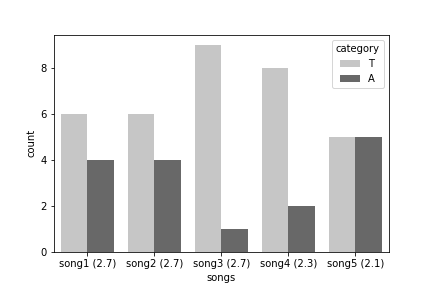
\includegraphics[width=0.485\textwidth]{songs_category.png}
    \caption{
        Bars show a count of the number of votes, respectively for
        Transfer-Americana and Americana, for each of the 5 songs.
        The numbers in parenthesis below the Bars is the average rating
        for each of the songs, when compared to a realistic human made
        song (1 is worst, 5 is best)
    \label{fig:songs}
    } 
\end{figure}

\begin{figure}
    \centering
    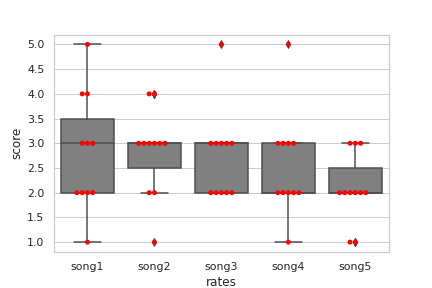
\includegraphics[width=0.485\textwidth]{scores.png}
    \caption{
        Boxplot of ratings for each of the 5 songs when compared to a realistic
        human made song (1 is worst, 5 is best). Median in horisontal black line,
        box defines by 25-75 percentile. The red dots are all registered scores.
        \label{fig:scores}
    }
\end{figure}

\subsubsection{Survey results}

\autoref{fig:songs} shows the count of the number of votes, respectively
for Transfer-Americana and Americana, for each of the 5 songs. The numbers in
parenthesis below the Bars is the average rating for each of the songs when
compared to a real human-made song (1 is worst, 5 is best). Inspecting the
figure we see a general trend where Transfer-Americana is favoured in 4 of 5
songs. Song 5 has a closer score and is also the song with the lowest average
rating of 2.1. 69 \% of all choices favour Transfer-Americana. A paired
t-test was conducted for this result, describing a significant favouring of
Transfer-Americana, with a p-value of 0.07. These results verified the
hypothesis that a music transformer model will perform better when it is
based on the pre-trained model, increasing the total number of music samples,
even though the base model was trained on the classical MAESTRO
dataset. It must be pointed out the uncertainty related to the relatively low
number of samples in the survey. In \autoref{fig:scores} a boxplot is
visualizing the single scorings in a more detailed manner. Red points mark
all the single scorings. The median for song 1 through 4 has a score of 3 and also
single scorings of 4 and 5, indicating that some people consider the songs as
comparable to human-made music.

In this survey some people have made comments about the overall performance,
focusing more on the subjective experience. A common comment were that the songs appear to all
get worse the longer they go on, as in the notes get more sparse and less
cohesive. The songs also seem to go all the way through a
scale. Such patterns make it very clear it is not a trained human playing
Another frequent comment was that it might have been better if the
songs from the different generators were shuffled for each question so the listeners
didn't naturally consider the differences between the two. This issue could 
color each opinion. Lastly it was the meaning of each 
rate in the scoring system was unclear related the human level of music composition.

\subsubsection{Expert Interviews}

Several samples of generated music were played for three
professional musicians and composers. All of these have degrees in
either music performance or composition, as well as experience with 
songwriting as well as performing music within a few of the subgenres of 
Americana, namely blues and folk. None of the musicians have any 
exprience or great knowledge of methods from ML or AI.

After a brief introduction to the concept of AI-generated music,
all of the musicians 
volunteered genres that would be easiest for a computer to generate. 
Classical music, especially baroque, blues and pop were all mentioned, 
as music within these genres ``have specific rules'' and that 
``there exists a recipe'' for these genres.
When asked if they could name genres that 
they thought would be difficult to model, jazz was the dominant response.
This initial hunch is interesting because 
it coincides with the space of genres that span the current work on music 
in AI.

The session proceded to listening to ten different pieces generated by our models.
They were organized in five pairs, such that each pair consisted of one 
piece of music generated by each of our two models.
The concensus amongst the musicians were that the music generated from 
the transfer-based model was best compared with the other model, but they
all emphasised that in absolute terms the generated music was not to be 
considered good.

From the discussion that followed after listening,
some general guidelines for music assessment can be 
extracted. Broadly summed up, one would like a musical piece to
``follow the rules'' both when it comes to rythm and scale, but also to 
``break the rules'' enough to make the piece interesting, but not 
chaotic. Preservation of long-term structure is important.
``It used the same stuff again!'', was loudly exclaimed 
by one of the musicians after a musical theme was repeated in one of the 
pieces.

Regarding scales and pitch variation, some interesting comments were 
made that exemplifies a common theme amongst our panel of experts;
\begin{displayquote}
"It sounds like a child, who has just learned a new scale, trying 
to remember which notes are correct by testing different ones." 
\end{displayquote}
The musician that made this comment was asked to elaborate and 
said that it is okay to venture outside the designated scale of the 
composition to create suspense, but that the generated music tended 
to do this very suddenly and without any transtion to the new 
regime. Moreover,
\begin{displayquote} 
``A structural break
can be nice to capture the attention of the listener, but you should
not overdo it''. 
\end{displayquote}
The musicians quickly adapted to a certain listening mindset, and
started counting ``errors'' the models made;
\begin{displayquote}
``In this piece there was 
only three scale breaches. Not too bad.''   
\end{displayquote}
Some musicians pointed to sections 
in the music that appeared to them as ``correct'' structural breaks, but 
though that the model seemed ``confuse itself'' by introducing them.

The musician thought that the models performance regarding rythm 
was wide-ranging, but seemed better than the ``scale rule-breaking''.
Some examples of grave rythmic errors were pointed out, for example
\begin{displayquote}
 ``That dotted note was incredibly weird!''   
\end{displayquote}
\begin{displayquote}
``What a very unexpected and
long rest.''   
\end{displayquote}

The results from the expert interviews are much in line with results described 
by \citeauthor{sturm2017taking} ~\cite{sturm2017taking}, collecting this kind 
of information from a website presenting generated 
music with RNN-based models. However, an important difference is the lack of 
desription of music background from the evaluators in that study. 

\section{Discussion}

Our goal nr 1 was to propose a framework for the evaluation of music generated
by machine learning with a Transformer architecture.
The combination of a quantitative system and two approaches to qualitative
evaluation is undoubtedly a step in this direction, giving a broader view of 
the results, also touching upon the more
subjective parts of an evaluation. We find that the guidelines provided by 
the musicians and the survey were in line with what the quantitative evaluation 
toolbox \lstinline|mgeval|~\cite{yang2020evaluation} is trying to 
do. However, we emphasise the need for such quantitative tools to have the basis
in an expert opinion as suggested by the ECD
framework~\cite{mislevy2003focus,mislevy2017evidence}.

A naturally related goal nr 2 of the work was to verify that a model trained by transfer
learning and therefore based on more samples will perform better, even though
the base model constitutes of songs of a different music genre, and as goal nr 3 show
that it is possible to generate more complex music than generated in earlier
related work. Results from qualitative and quantitative evaluation clearly
show that Transfer-Americana perform better than Americana, fulfilling goal
2. Scorings from comparison with human-made music to some degree supports
goal 3, with an average rating of 2.6 of 5, but there is still a way to go.
Especially for the songs from the Americana model, we see that the melodic
part degrades faster than for Transfer-Americana, a pattern which probably has
affected the comparisons and the scoring.

An interesting pattern is the variation in count of superiority between songs
in figure \ref{fig:songs}. In song 1-4, the count shows a clear overweight on
Transfer-Americana, especially evident for song 3 and 4. For song 5 the count
is close to similar. When we compare this to the technical evaluation there is 
support in this pattern for song 1-4. For song 3 and 4 there is a longer distance 
between Americana and Transfer-Americana and the difference between the 2 versions 
should be higher. It could be that the composition and complexity in
certain primers are more dependent on a bigger database of trained songs, than
other primers. This is something to further analyse in future work. Scorings
in figure \ref{fig:scores} return many 3's and some 4's and 5's, but also
1's, indicating that some people think this is truly realistic music, while
others condsider human-made and generated music as two different worlds.

Processing of data and adapting a framework to fit our problem 
took an extraordinary amount of time. Optimally the models should have been
trained for a longer period, and the resulting model is a minimal viable model.
Transformer models can be monstrous 
an unwieldy structures, illustrated by this quote from
\citeauthor{vaswani2017attention}: ``The Transformer allows for significantly
more parallelization and can reach a new state of the art in translation
quality after being trained for as little as twelve hours on eight P100 GPUs''.
We find it odd to assume that it is normal to have access to a rack of eight 
professional-grade GPUs~\cite{vaswani2017attention}, illustrating the importance
of further development of the transformer to increase the efficiency 
\cite{kitaev2020reformer}.

\section{Conclusions and further development}

An evaluation framework spanning over quantitative and qualitative techniques
give a broader evaluation basis for music generated by machine learning 
based on the transformer architecture. Utilizing this framework to evaluate two different 
approaches for generating Americana music gave confidence in the superiority of a 
transfer learning based model (trained on the MAESTRO dataset) over a model solely
trained on the Americana dataset.

Resulting songs generated by three-bar Americana primers was to some degree evaluated to 
be relatively close to human made music, with major differences between different melodies.
However, the number of samples in the different evaluation approaches was relatively small. 
To increase the confidence in the results, a further work will be to massively scale up, both the 
number of generated songs for the the technical evaluation and the number of persons in the 
qualitative analysis.

We think that interviews with composers and musician about what makes ``good'' music 
is warranted. Moreover, we find it interesting to present AI-generated 
music to musical experts in the manner we have done to be particularly beneficial. 
An extension of this venue of research to consist of individual interviews
and also contain a sort of ``musical Turing test'' is natural. As mentioned in 
chapter V, some form of systematic interviews has been utilized by \citeauthor{sturm2017taking} 
\cite{sturm2017taking}, but when we combine this approach with the other 2 evaluation
metrics described in this paper, the resulting framework becomes novel and more robust as an
evaluation method for machine learning methods in the creative arts domain, such as music.

\vspace{3em}

\printbibliography

\end{document}